% Scene A of "Render a ping without Gazebo" (render-a-ping.md), from gz_sonar/examples/render_ping.cc:
% imaging sonar (ECHO, 700 kHz, 120 x 20 deg, 10 m window), level, 3 m deep; a 0.25 m sphere 5 m ahead on the axis;
% seabed 7 m below the sonar. Side view, true scale, 1 unit = 1 m.
% Build: pdflatex render_ping_A.tex, then pdftocairo to ../images/render_ping_A.{png,svg}
\documentclass[tikz,border=6pt]{standalone}
\usetikzlibrary{arrows.meta,calc}
\renewcommand{\familydefault}{\sfdefault}
\tikzset{
  lbl/.style={font=\sffamily\small},
  beam/.style={fill=black!7,draw=black,thin},
  dim/.style={thin,{Latex[length=1.6mm]}-{Latex[length=1.6mm]}},
  lead/.style={thin,black!70},
  axis/.style={thin,dashed},
  shadow/.style={fill=black!30,draw=none},
}
% seabed line from x0 to x1 at height z (drawing units), slab of dots below
\newcommand{\seabed}[3]{
  \draw[thick] (#1,#3) -- (#2,#3);
  \foreach \r [count=\i] in {0.12,0.3} {
    \pgfmathsetmacro{\o}{mod(\i,2)*0.12}
    \pgfmathsetmacro{\n}{int((#2-#1-0.3)/0.24)}
    \foreach \k in {0,...,\n} \fill ({#1+0.12+\k*0.24+\o},{#3-\r}) circle (0.4pt);
  }
}
% sonar head at #1, pitched down #2 degrees
\newcommand{\head}[2]{
  \begin{scope}[shift={#1},rotate=-#2]
    \draw[fill=black!15] (-0.5,-0.13) rectangle (0,0.13);
    \fill (0,0) circle (1.4pt);
  \end{scope}
}
\begin{document}
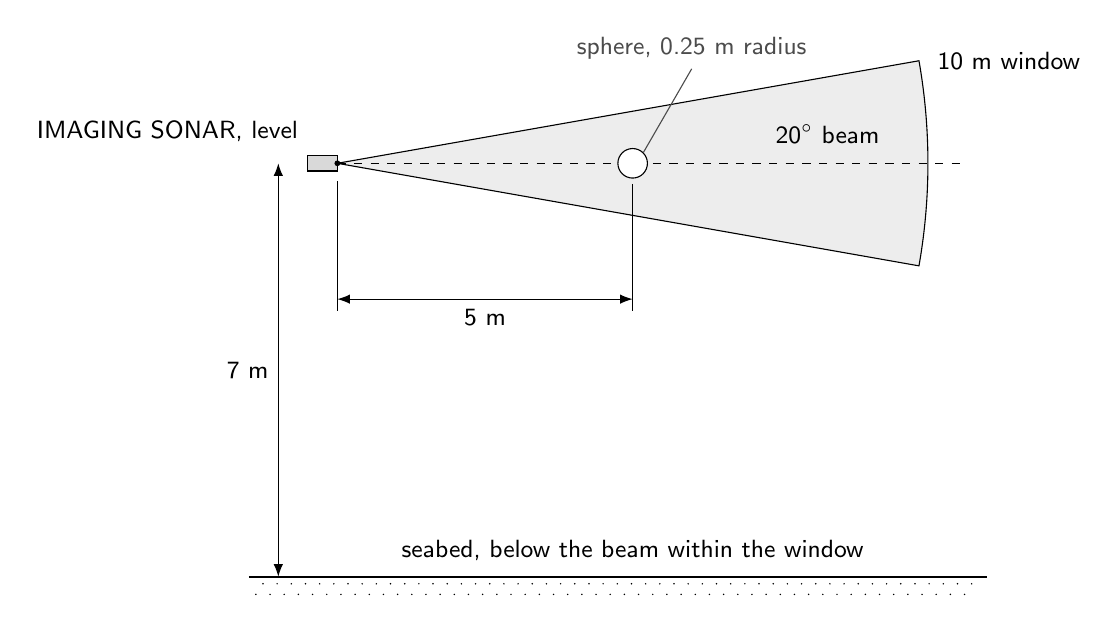
\begin{tikzpicture}[scale=0.75]
  \seabed{-1.5}{11}{-7}
  % beam, 20 deg tall, out to the 10 m window
  \draw[beam] (0,0) -- ({10*cos(10)},{10*sin(10)}) arc (10:-10:10) -- cycle;
  \draw[axis] (0,0) -- (10.6,0);
  \draw[fill=white] (5,0) circle (0.25);
  \head{(0,0)}{0}
  % dimensions
  \draw[dim] (0,-2.3) -- (5,-2.3) node[lbl,midway,below] {5 m};
  \draw (0,-0.3) -- (0,-2.5) (5,-0.35) -- (5,-2.5);
  \draw[dim] (-1,0) -- (-1,-7) node[lbl,midway,left] {7 m};
  \node[lbl,anchor=west] at ({10*cos(10)+0.15},{10*sin(10)}) {10 m window};
  \node[lbl] at (8.3,0.5) {20$^\circ$ beam};
  \draw[lead] (5.18,0.18) -- (6,1.6) node[lbl,anchor=south] {sphere, 0.25 m radius};
  \node[lbl,anchor=south east] at (-0.5,0.2) {IMAGING SONAR, level};
  \node[lbl,anchor=south] at (5,-6.9) {seabed, below the beam within the window};
\end{tikzpicture}
\end{document}
